\chapter{Spark应用启动过程分析}
\label{cha:run_wordcount}
\section{WordCount程序}
\label{sec:spark_wd}
阅读Spark源码以Spark集群中运行WordCount应用顺序为根据,理解出Spark应用运行的流程,从而达到阅读源码的目的。

本WordCount源码如程序\ref{lst:spark_wd}所示:

\begin{lstlisting}[
caption = {基于Spark的WordCount程序},
label={lst:spark_wd},
language = Scala
]
package org.apache.spark.examples
import org.apache.spark.{SparkConf, SparkContext}
object HelloWorld {
def main(args: Array[String]): Unit = {
    val scf = new SparkConf();
    scf.setAppName("Spark Count")
    val sc = new SparkContext(scf)
    val scfclone = sc.getConf
    val threshold = args(1).toInt
    val tokenizde = sc.textFile(args(0)).flatMap(_.split(" "))
    println("tokenizde: " + tokenizde)
    val wordCount = tokenizde.map((_, 1)).reduceByKey(_ + _)
    println("wordCount: " + wordCount)
    val filtered = wordCount.filter(_._2 >= threshold)
    val charCount = filtered.flatMap(_._1.toCharArray).map((_,1)).reduceByKey(_+_)
    println(filtered.collect().mkString(","))
  }
}
\end{lstlisting}

将输入案例input.txt放入hdfs中,已搭建好环境的Spark集群,打包好的WordCount jar包且提交到集群中的任意一台机器(本例中为master)中。

\section{提交WordCount程序}
\label{sec:submit_app}
程序提交的整个过程如图\ref{spark-submit}所示:
\begin{figure}[H] % use float package if you want it here
	\centering
	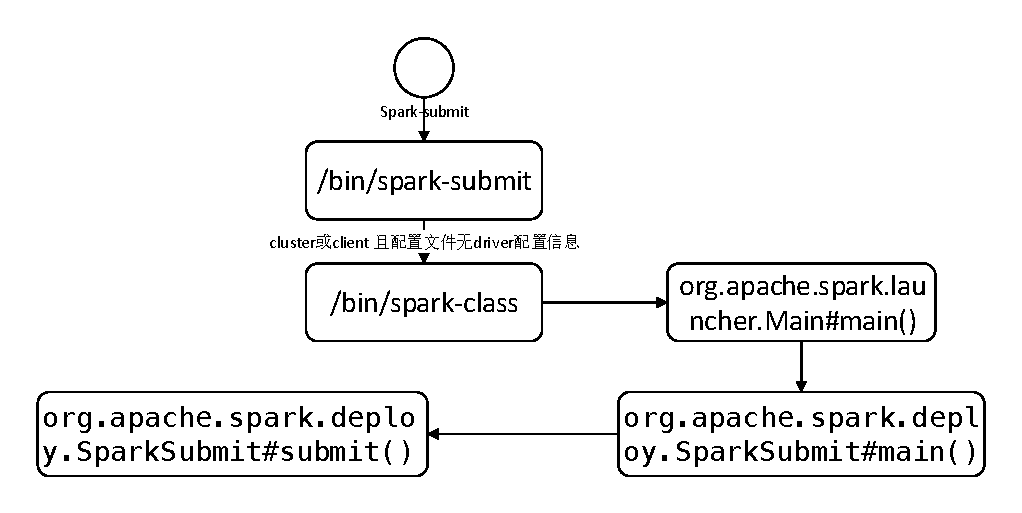
\includegraphics{figures/sparksubmit.pdf}
	\caption{spark-submit运行流程}
	\label{spark-submit}
\end{figure}

在master中运行提交命令如下:
	
\begin{cmd}
/usr/bin/spark-submit
   HelloWorld-1.0-SNAPSHOT-jar-with-dependencies.jar
   /user/inputfile.txt 2
\end{cmd}

从这条命令可以看出使用的是spark-submit shell脚本,后面三个为参数,第一个为目录下的WordCount jar包,第二个为hdfs中的输入文件,第三个为WordCount中限定输出的value临界值。
我们打开spark-submit shell脚本,脚本如所示。

spark-submit shell脚本内容如程序\ref{lst:sparksubmit}所示。

\begin{lstlisting}[
caption = {spark-submit.sh脚本},
label={lst:sparksubmit},
language = sh
]
SPARK_HOME="$(cd "`dirname $(readlink -nf "$0")`"/..; pwd -P)"
export PYTHONHASHSEED=0
exec "SPARK_HOME"/bin/spark-class org.apache.spark.deploy.SparkSubmit "$@"

\end{lstlisting}

从程序\ref{lst:sparksubmit}可以看出,spark-submit执行流程是:首先找出Spark安装的根目录,然后再去执行spark-class这个shell脚本,参数为org.apache.spark.deploy.SparkSubmit以及提交命令后跟的所有参数。

spark-class脚本先找到master的java,遍历Spark安装目录下lib目录下的jar包,加入到CLASSPATH中,具体内容如下:

\begin{centertitlebox}{spark-class的CLASSPATH值}
/usr/hdp/current/spark-historyserver/conf/\\
/usr/hdp/2.4.0.0-169/spark/lib/spark-assembly-1.6.0.2.4.0.0-169-hadoop2.7.1.2.4.0.0-169.jar\\
/usr/hdp/2.4.0.0-169/spark/lib/datanucleus-api-jdo-3.2.6.jar\\
/usr/hdp/2.4.0.0-169/spark/lib/datanucleus-core-3.2.10.jar\\
/usr/hdp/2.4.0.0-169/spark/lib/datanucleus-rdbms-3.2.9.jar\\
/usr/hdp/current/hadoop-client/conf/
\end{centertitlebox}

spark-class最后通过Java -cp $\left\langle \textit{classpath} \right\rangle$ org.apache.spark.launcher.Main 参数列表,
开启jvm进程,执行的主类为org.apache.spark.launcher.Main,传过来的参数有:
\begin{itemize} 
	\item[---] org.apache.spark.deploy.SparkSubmi
	\item[---] HelloWorld-1.0-SNAPSHOT-jar-with-dependencies.jar
	\item[---] /user/inputfile.txt
\end{itemize}

最后启动的Java程序的命令如下:
\begin{centertitlebox}{spark-class创建的Java虚拟机命令}
 java -Dhdp.version=2.4.0.0-169\\
	 -cp <classpath>\\
	 -Xms1g -Xmx1g\\
	 org.apache.spark.deploy.SparkSubmit\\
	 --master yarn\\ 
	 --deploy-mode client\\
	 HelloWorld-1.0-SNAPSHOT-jar-with-dependencies.jar\\
	 /user/inputfile.txt 2
\end{centertitlebox}

\section{准备WordCount提交程序运行环境}
\label{sec:runmain}

org.apache.spark.launcher.Main代码片段如程序\ref{lst:launchermain}所示。
传入此类的main方法的参数有:
\begin{itemize}
	\item org.apache.spark.deploy.SparkSubmit
	\item --master yarn-client
	\item HelloWorld-1.0-SNAPSHOT-jar-with-dependencies.jar
	\item /user/inputfile.txt
\end{itemize}
代码通过SparkSubmitCommandBuilder方法生成相应的Java命令,然后返回给cmd,
最后程序判断运行的主机是Windows还是bash,打印到控制台,之后spark-class脚本
重定位到这里并读取输出的字符流\footnote{launcher.Main函数在spark-class
脚本中执行,spark-class脚本会读取Main的标准输出,将标准输出解析为启动程序命令。},
通过exec执行java命令。
\begin{lstlisting}[%
language = Java,
caption = {launcher.Main程序代码片段},
label = {lst:launchermain}
]
public static void main(String[] argsArray) throws Exception {
	List<String> args = new ArrayList<>(Arrays.asList(argsArray));
	String className = args.remove(0);
	AbstractCommandBuilder builder;
	if (className.equals("org.apache.spark.deploy.SparkSubmit")) {
	try {
	  builder = new SparkSubmitCommandBuilder(args);
	} catch (IllegalArgumentException e) { ... }
	
	Map<String, String> env = new HashMap<>();
	List<String> cmd = builder.buildCommand(env);	
	if (isWindows()) {
		System.out.println(prepareWindowsCommand(cmd, env));
	} else {
		// In bash, use NULL as the arg separator since it cannot be used in an argument.
		List<String> bashCmd = prepareBashCommand(cmd, env);
		for (String c : bashCmd) {
			System.out.print(c);
			System.out.print('\0');
		}
	}
}
\end{lstlisting}
\section{进入Spark-Submit提交主类}
\label{SparkSubmitMain}
前面的准备工作工作后最后调用org.apache.spark.deploy.SparkSubmit类的main方法,程序代码如程序\ref{sparksubmitmainscala}所示
\begin{lstlisting}[%
language=Scala,
caption={SparkSubmit.scala中main函数},
label={sparksubmitmainscala}]
	def main(args: Array[String]): Unit = {
	val appArgs = new SparkSubmitArguments(args)
	if (appArgs.verbose) {
	// scalastyle:off println
	   printStream.println(appArgs)
	// scalastyle:on println
	}
	appArgs.action match {
	    case SparkSubmitAction.SUBMIT => submit(appArgs)
    	case SparkSubmitAction.KILL => kill(appArgs)
	    case SparkSubmitAction.REQUEST_STATUS => requestStatus(appArgs)
	  }
	}
\end{lstlisting}
首先第一步是构造参数;第二步是根据提供的参数匹配相应的操作。
\begin{enumerate}[\bfseries 1]
   \item 构造提交参数方法
       \begin{enumerate}
       	 \item 将提交脚本中的参数做个转换,像—master等;
       	 \item 合并—conf中和spark-default.conf中的参数;
       	 \item 删掉不是是spark系统的配置参数;
       	 \item 从环境脚本中读入默认配置参数并合并;
       	 \item 验证配置参数的有效性;
       \end{enumerate}
   \item 提交
   参数中的action默认为SUBMIT,所以这步会执行submit方法。
   该方法中有两个较为重要的方法
   \begin{centertitlebox}{SparkSubmit调用的两个重要的方法}
   	val (childArgs, childClasspath, sysProps, childMainClass) = prepareSubmitEnvironment(args)\\
   	runMain(childArgs, childClasspath, sysProps, childMainClass, args.verbose)
   \end{centertitlebox}
     \begin{enumerate}
     	\item 对于prepareSubmitEnvironment
     	此方法返回一个较为重要的参数即childMainClass,其会根据deploy-mode
     	对应不同的实现,具体如图\ref{prepareSubmit}所示
        	\begin{figure}[H] 
     		\centering
     		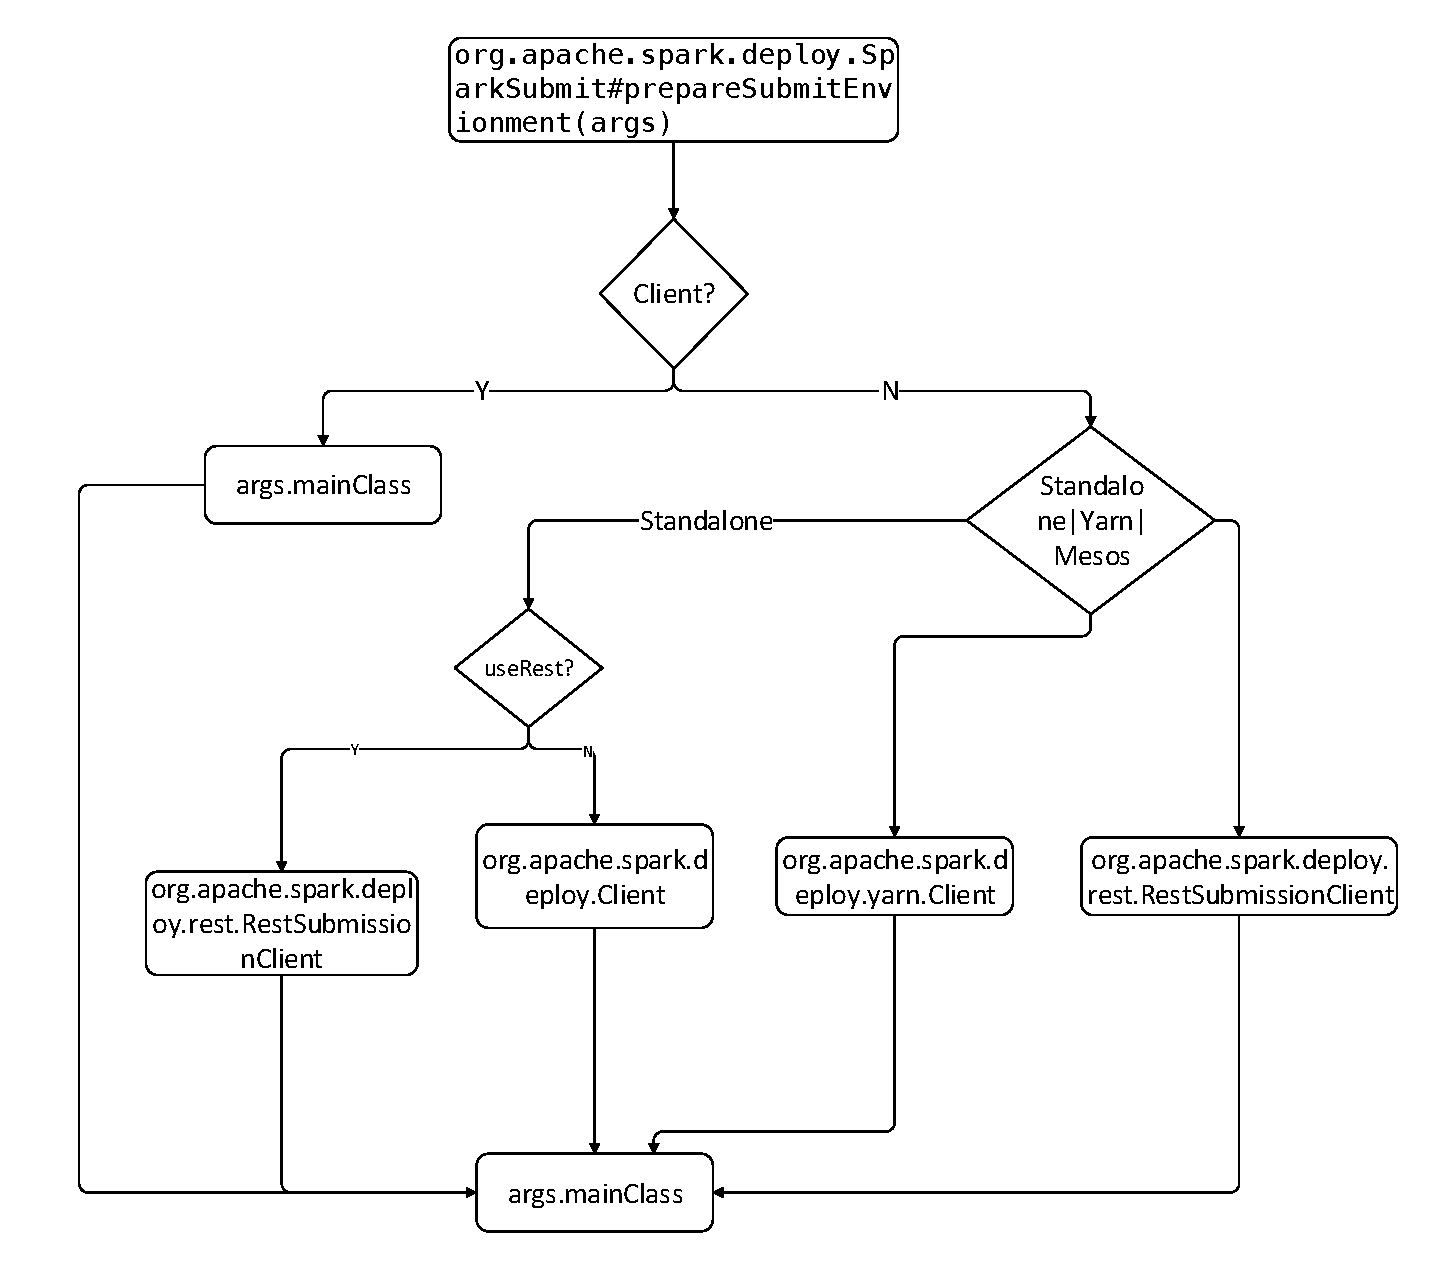
\includegraphics[scale=0.55]{figures/prepareSubmit.pdf}
     		\caption{prepareSubmit运行流程}
     		\label{prepareSubmit}
        	\end{figure}
为了验证自己分析的正确性,通过中间输出调试的方式,分别输出了在yarn-cluster和yarn-client模式下该方法返回的四元组值,命令为最前面的命令,其结果如表\ref{tab:deploymode}所示
           \begin{table}[t]
           	\caption{Yarn-Cluster和Yarn-Client模式下的参数对比}
      		\label{tab:deploymode}
      		\begin{tabularx}{\linewidth}{p{2.5cm}XX}
      			\toprule[1.5pt]
      			{\heiti 参数名} & {\heiti Yarn-Cluster} &{\heiti Yarn-Client}\\
      			\midrule[1pt]
      		childArgs&&ArrayBuffer(/user/root/inputfile.txt, 2)\\
      		childClasspath&ArrayBuffer()&ArrayBuffer(file:/root/HelloWorld-1.0-SNAPSHOT-jar-with-dependencies.jar)\\
      		sysProps&很多,基本都是系统属性&spark.master->yarn-client\\
      		childMainClass&org.apache.spark.deploy.yarn.Client&com.wtx.HelloWorld\\
      		\bottomrule[1.5pt]
      		\end{tabularx}
          \end{table}
       由结果可知,我们的分析是正确的。
       这里我们使用的master为yarn,deploy-mode为cluster,所以childMainClass为org.apache.spark.deploy.yarn.Client。
       \item 对于runMain
       \begin{enumerate}
       	\item 先检查查是否可见,是的话打印出各个参数的配置信息;
       	\item 跟据spark.driver.userClassPathFirst这个属性确定类加载器,这个属性可以降低Spark依赖和用户依赖的冲突。它现在还是一个实验性的特征;
       	\item 将jar包加入到类加载器的classpath;
       	\item 通过反射射的方式找到mainClass,然后在获得其main方法,并通过invoke加载main方法,这里就是org.apache.spark.deploy.yarn.Client的main方法。
       \end{enumerate}
     \end{enumerate}
\end{enumerate}
    到这里spark-submit就执行完了,接下来将分析org.apache.spark.deploy.yarn.Client的main方法执行过程。
\section{Yarn代理的启动}
由\ref{SparkSubmitMain}节我们知道,其最后就是反射加载org.apache.spark.deploy.yarn.Client的main方法,其执行过程如图\ref{fig:YarnClientMain}所示
	\begin{figure}[H] 
	\centering
	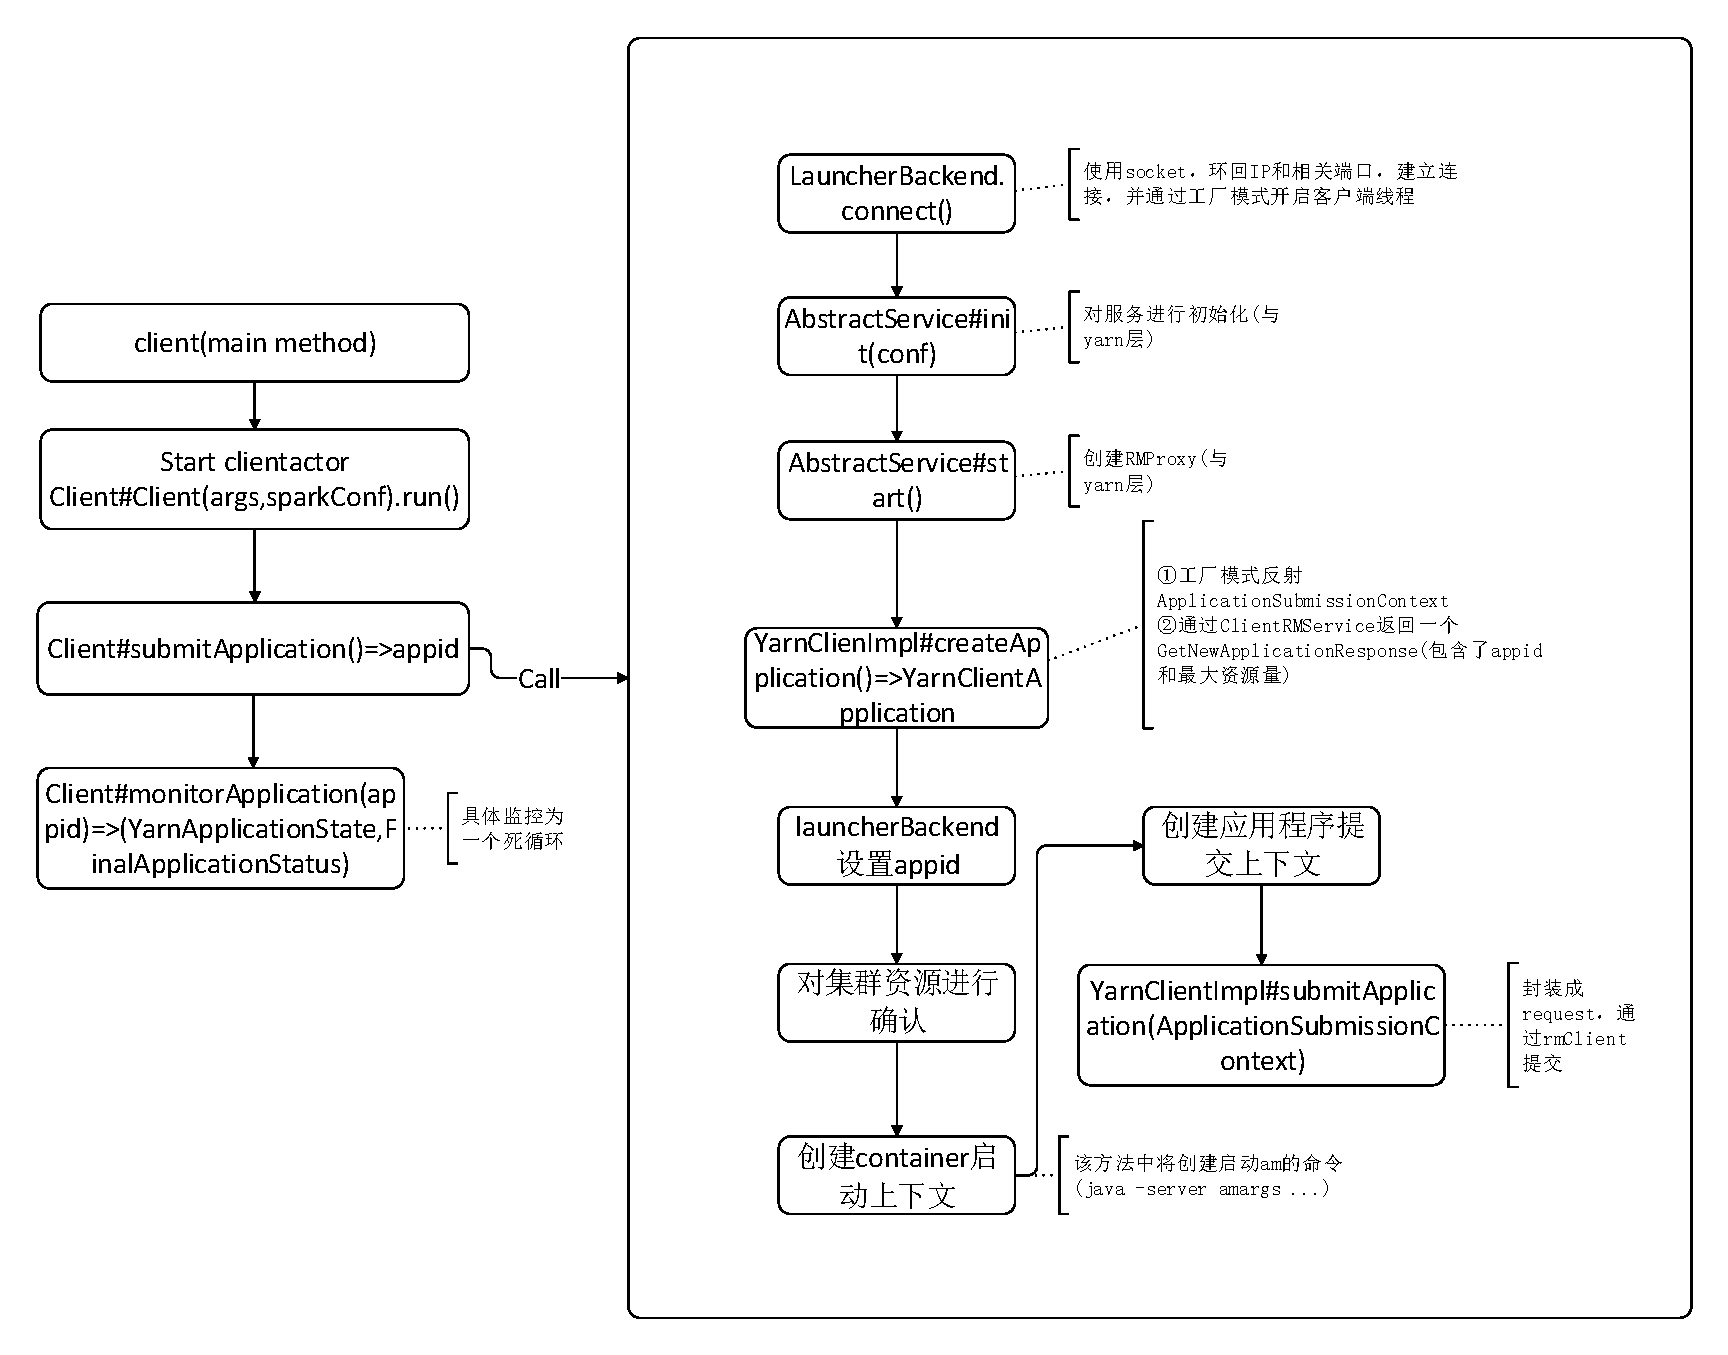
\includegraphics[width=\textwidth]{figures/YarnClientMain.pdf}
	\caption{YarnClientMain流程}
	\label{fig:YarnClientMain}
\end{figure}
main函数代码如程序\ref{fig:yarnclientmainscala}所示
\begin{lstlisting}[%
language=Scala,
caption={YarnClient中main函数},
label={fig:yarnclientmainscala}]
/**
* --name, com.wtx.HelloWorld,
* --jar, file:/root/HelloWorld-1.0-SNAPSHOT-jar-with-dependencies.jar,
* --class, com.wtx.HelloWorld,
* --arg, /user/root/inputfile.txt,
* --arg, 2
* */
def main(argStrings: Array[String]) {
	if (!sys.props.contains("SPARK_SUBMIT")) {
	logWarning("WARNING: This client is deprecated and will be removed in a " +
		"future version of Spark. Use ./bin/spark-submit with \"--master yarn\"")
	}
	System.setProperty("SPARK_YARN_MODE", "true")
	val sparkConf = new SparkConf
	val args = new ClientArguments(argStrings, sparkConf)
	if (!Utils.isDynamicAllocationEnabled(sparkConf)) {
		sparkConf.setIfMissing("spark.executor.instances", args.numExecutors.toString)
	}
	new Client(args, sparkConf).run()
}
\end{lstlisting}
这里面第一个执行的是ClientArguments方法,该方法中
\begin{itemize}
	\item[---] 对传入的参数进行解析,通过—标识符识别,像jar、class、arg之类的
	\item[---] 获取spark环境中的默认配置参数,就是获取spark.yarn.dist.files和spark.yarn.dist.archives这两个
	\item[---] 对已经解析出来的参数进行校验
\end{itemize}

之后就是Client中的主要方法,new Client(args, sparkConf).run()。

创建Client对象时,对一些变量如yarnClient、amMemoryOverhead、executorMemoryOverhead、isClusterMode等,其中yarnClient初始化为YarnClientImpl对象。
接着就是运行run方法。其代码如程序\ref{yarnclientrunscala}所示
\begin{lstlisting}[%
language=Scala,
caption={YarnClient中run函数},
label={yarnclientrunscala}]
def run(): Unit = {
	this.appId = submitApplication()
	if (!launcherBackend.isConnected() && fireAndForget) {
    	val report = getApplicationReport(appId)
    	val state = report.getYarnApplicationState
    	logInfo(s"Application report for $appId (state: $state)")
    	logInfo(formatReportDetails(report))
    	if (state == YarnApplicationState.FAILED || state == YarnApplicationState.KILLED) {
			throw new SparkException(s"Application $appId finished with status: $state")
		}
	} else {
    	val (yarnApplicationState, finalApplicationStatus) = monitorApplication(appId)
    	if (yarnApplicationState == YarnApplicationState.FAILED ||
      		finalApplicationStatus == FinalApplicationStatus.FAILED) {
     		 throw new SparkException(s"Application $appId finished with failed status")
    	}
    	if (yarnApplicationState == YarnApplicationState.KILLED ||
			finalApplicationStatus == FinalApplicationStatus.KILLED) {
      		throw new SparkException(s"Application $appId is killed")
    	}
    	if (finalApplicationStatus == FinalApplicationStatus.UNDEFINED) {
      		throw new SparkException(s"The final status of application $appId is undefined")
    	}
	}
}
\end{lstlisting}

run里第一个调用的方法就是Client\#submitApplication()方法,此方法最终返回的是与yarn通信之后的applicationId。
Client\#submitApplication()方法主要作用如下
\begin{itemize}
	\item launcher server进行连接
	\item   对sparkconf初始化,并创建对ResourceManager的代理客户端rmClient,以及开启historyClient和timelineClient(具体怎么建立代理会在下一部分详述,这里我们只需要理解成客户端操作服务端的方法就像操作本地的方法一样)
	\item 调用YarnClientImpl\#createApplication()与yarn上创建一个YarnClientApplication对象,其类图如图\ref{YarnClientApplication}所示,这里面包含了重要的appid等信息
		\begin{figure}[H] 
		\centering
		
\includegraphics{figures/YarnClientApplication.pdf}
		\caption{YarnClientApplication类图}
		\label{YarnClientApplication}
	\end{figure}
	\item 核对集群上是否满足ApplicationMaster的资源要求
	\item 创建ApplicationMaster的Container启动上下文信息,这里面将上传三种文件到hdfs对应的目录,分别为spark-hdp-assemably、我们编写的spark应用jar包以及spark配置信息,之后将为amContainer封装一个启动AM\footnote{AM为ApplicationMaster的简写,以后本文中的AM不做特殊说明,均指代ApplicationMaster}的命令,类似于java -server 这样的
	\item 创建提交AM的上下文信息,包括spark应用名称、AM内存以及扩展值、AM虚拟核数等信息
	\item 将AM上下文信息提交到ResourceManager
\end{itemize}

run里面第二个调用就是monitorApplication(ApplicationId)。此函数通过Client\#submitApplication()方法返回的appid实现对提交spark应用的监控,在实现上通过一个死循环,让客户端线程每隔spark.yarn.report.interval中定义的时间进行应用执行状态的获取,然后显示在客户端控制台上。应用执行状态(ACCEPTED之后)即为以下四种的一种,FINISHED, FAILED,KILLED或者RUNNING。程序最终执行状态定义为以下四种UNDEFINED, SUCCEEDED, FAILED或KILLED。
\section{ApplicationMaster的启动}
前面通过yarn的代理客户端提交文件和提交程序信息之后,由yarn来进行分配container\footnote{container为资源的抽象,包含CPU、内存、网络资源和硬盘,Yarn中负责分配CPU和内存}给am,并将am的上下文信息发送给包含amContainer的nodeManager,由其来启动am。am的main函数如程序\ref{ammain}所示
\begin{lstlisting}[%
language=Scala,
caption={ApplicationMaster中main函数},
label={ammain}]
def main(args: Array[String]): Unit = {
	SignalLogger.register(log)
	val amArgs = new ApplicationMasterArguments(args)
	SparkHadoopUtil.get.runAsSparkUser { () =>
    	master = new ApplicationMaster(amArgs, new YarnRMClient(amArgs))
    	System.exit(master.run())
	}
}
\end{lstlisting}

在spark源码中am由单例对象和伴生类组成,main函数的处理过程如下
\begin{itemize}
	\item 对传入am的参数进行解析封装成ApplicationMasterArguments,其类图如图\ref{ApplicationMasterArguments}所示
\begin{figure}[H] 
	\centering
	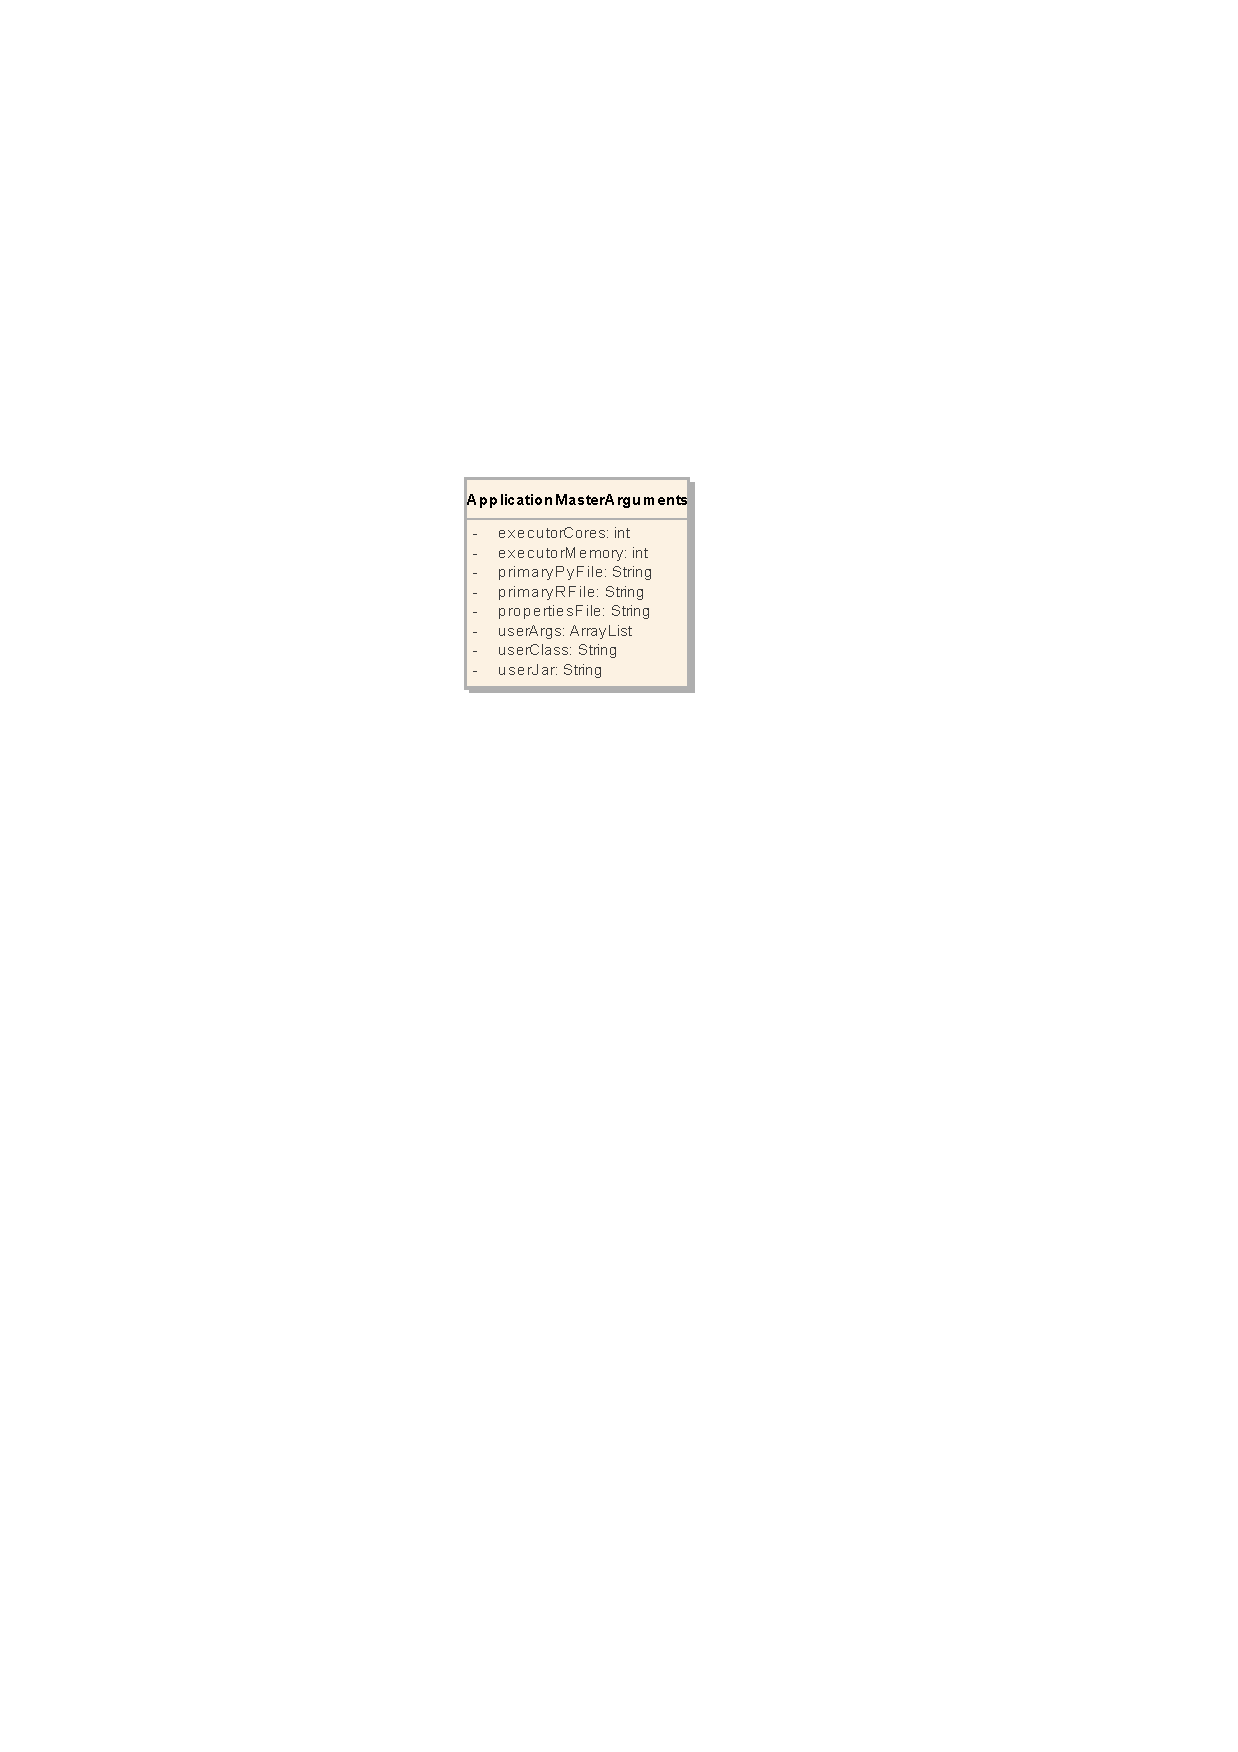
\includegraphics{figures/ApplicationMasterArguments.pdf}
	\caption{ApplicationMasterArguments类图}
	\label{ApplicationMasterArguments}
\end{figure}
	\item 实例化ApplicationMaster,这里实例的是ApplicationMaster的伴生类,因为单例对象是不能实例化的,且我们要注意实例化ApplicationMasterArguments
	ApplicationMaster传入的第二个参数为YarnRMClient,这个负责在yarn上注册或者取消Application
	\item 执行ApplicationMaster的run方法,此方法首先获取yarn的配置信息,然后对Application进行注册,接着判断是否为cluster模式,是的话就是启动driver,否则启动executor
\end{itemize}
\section{Driver的启动}
Yarn-Cluster模式下Driver的启动过程如图\ref{fig:startDriver}所示
\begin{figure}[H]
	\centering
		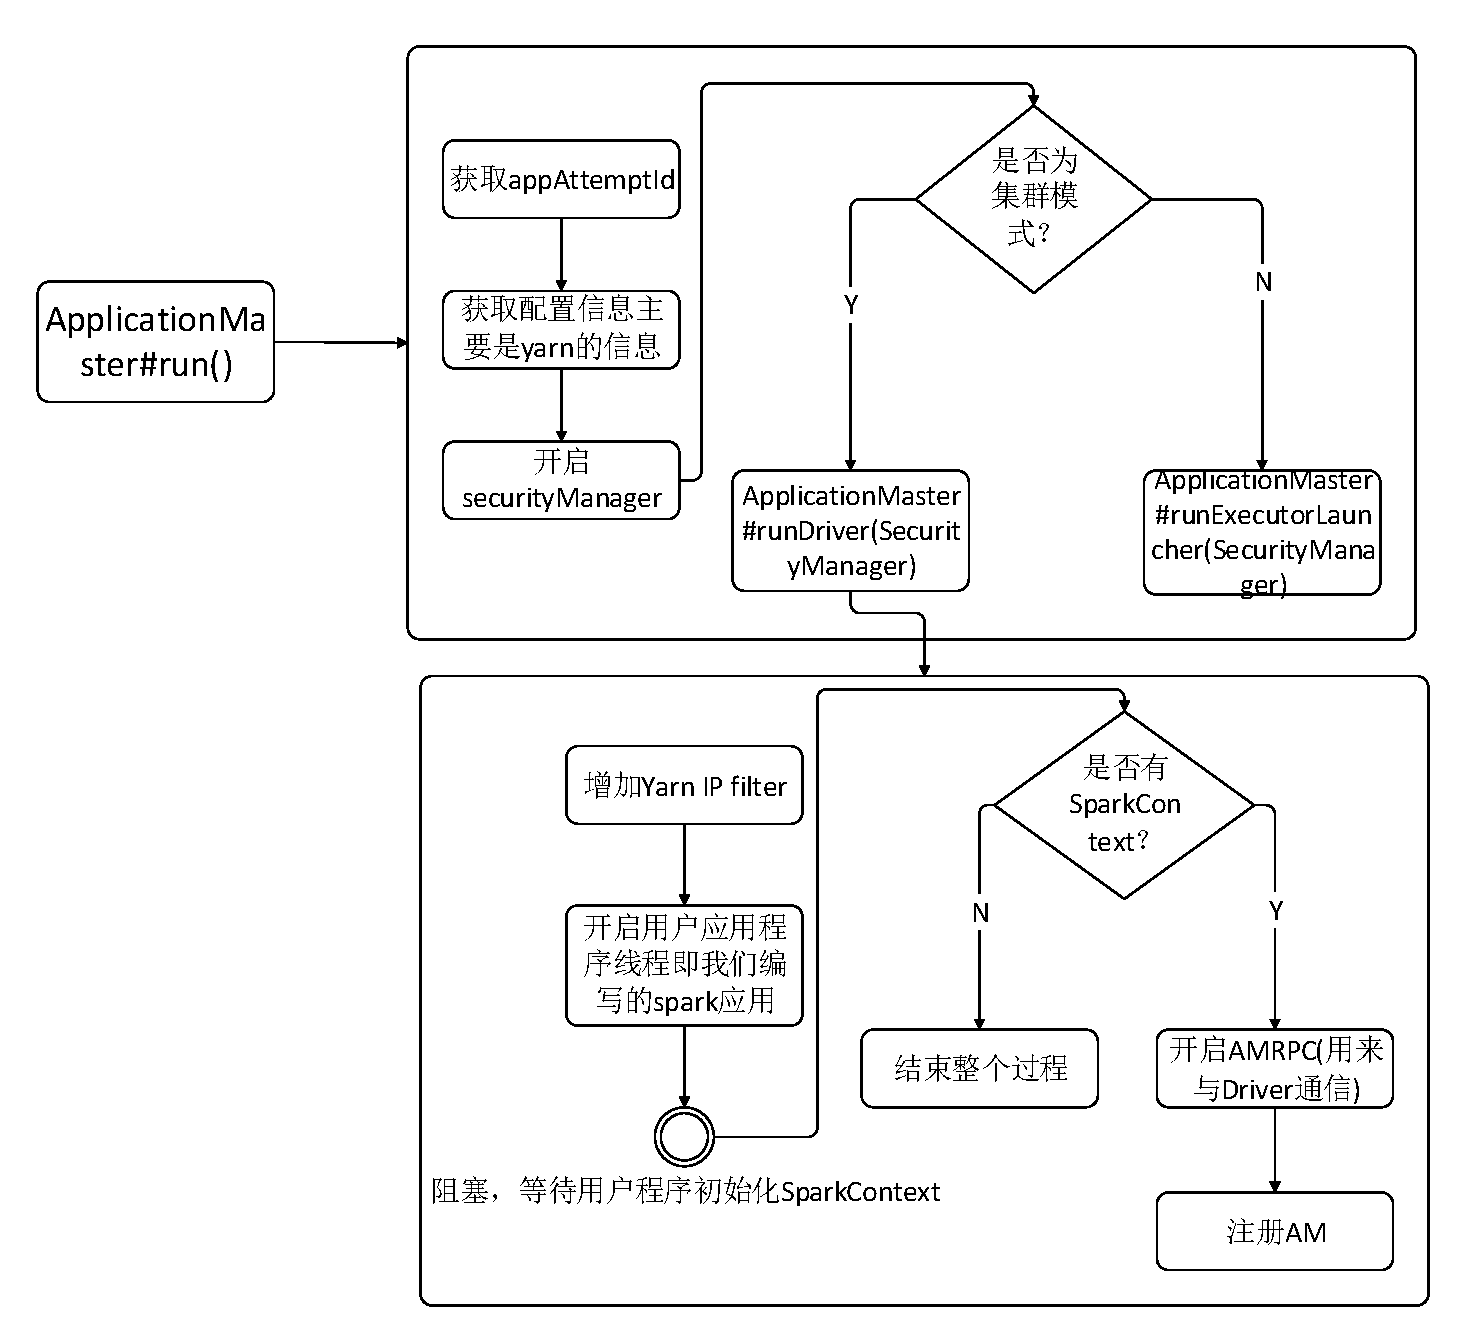
\includegraphics[width=\textwidth]{figures/startDriver.pdf}
	\caption{Driver启动过程}
	\label{fig:startDriver}
\end{figure}

启动Dirver的程序如程序\ref{lst:rundriver}所示
\begin{lstlisting}[%
language=Scala,
caption={启动Driver},
label={lst:rundriver}]
private def runDriver(securityMgr: SecurityManager): Unit = {
    addAmIpFilter()
    userClassThread = startUserApplication()
    val sc = waitForSparkContextInitialized()
    if (sc == null) {
        finish(FinalApplicationStatus.FAILED,
        ApplicationMaster.EXIT_SC_NOT_INITED,
        "Timed out waiting for SparkContext.")
    } else {
        rpcEnv = sc.env.rpcEnv
        val driverRef = runAMEndpoint(
        sc.getConf.get("spark.driver.host"),
		sc.getConf.get("spark.driver.port"),
		isClusterMode = true)
		registerAM(rpcEnv, driverRef, sc.ui.map(_.appUIAddress).getOrElse(""), securityMgr)
		userClassThread.join()
	}
}
\end{lstlisting}

从源码中可以看到启动Driver的第一步为启动用户程序\footnote{这里的用户程序即为我们所编写的WorldCount程序},这里面对启动用户程序做了配置,具体如下
\begin{itemize}
	\item 获得用户程序所需要的ClassPath
	\item 获取类加载器信息
	\item 获得用户jar包路径
	\item 获得用户程序主类参数列表
	\item 开启一个新的线程,通过反射机制,以用户程序主类主函数为入口,加载用户程序
\end{itemize}

在用户程序主类的运行过程中,此时主线程\footnote{指AM进程中运行Driver的线程}会阻塞,等待用户程序SparkContext初始化完成。